Cette partie de l'application est principalement basée sur l'analyse et l'enregistrement des notes jouées par 
l'utilisateur. Le principe est d'analyser en temps réel les fréquences à la base du son de la guitare, et de faire en sort de constituer un accord
avec les notes ayant le volume le plus fort et l'enregistrer. De plus, le modèle comporte également toutes les informations sur les préférences
de l'utilisateur pour l'application,   ainsi que des fonctions pour enregistrer les données. Nous avons choisi de sauvegarder les fichiers au format JSON.\newline

\begin{figure}[H]
\centering
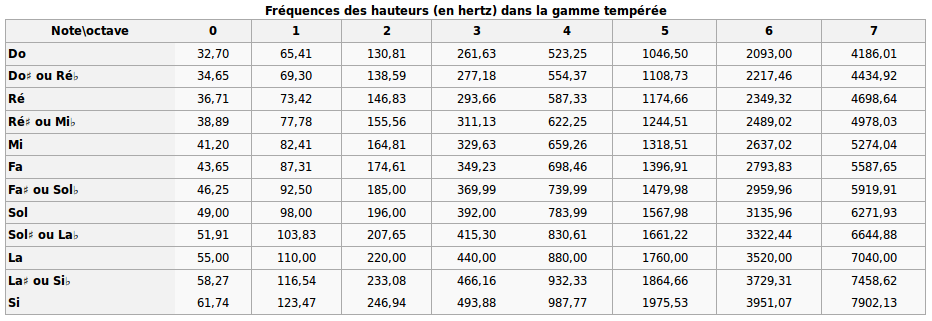
\includegraphics[scale=0.5]{Frequences}
\caption{Toutes les frequences possibles}
\end{figure}